\subsubsection{MLP Results}

Recalling the implemented methodology, the chosen architecture consists of two hidden layers: the first with 64 neurons and the second with 32 neurons. Using this architecture, the following results were obtained:

\begin{figure}[H]
    \centering
    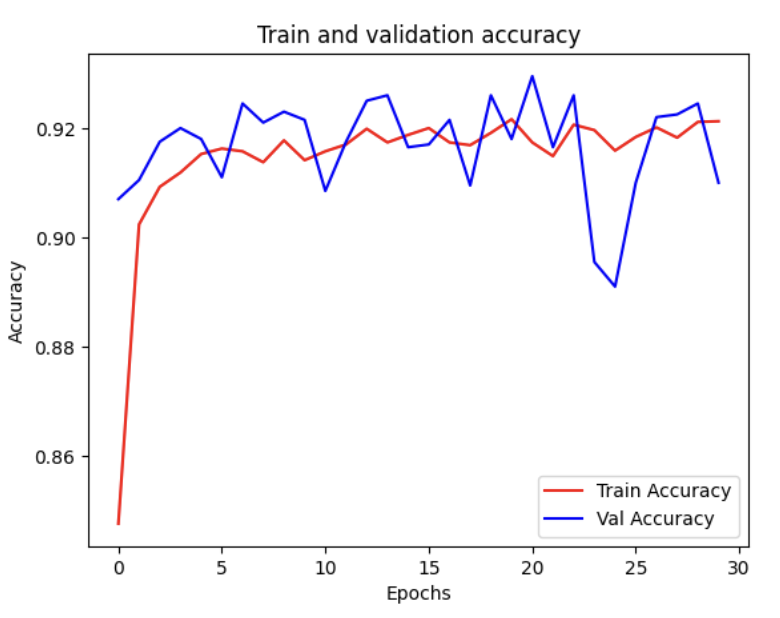
\includegraphics[width=\linewidth]{images/mlp_accuracy_training_And_Validation.png}
    \caption{Accuracy during training and validation for the MLP model.}
    \label{fig:mlp_accuracy_training_validation}
\end{figure}

\begin{figure}[H]
    \centering
    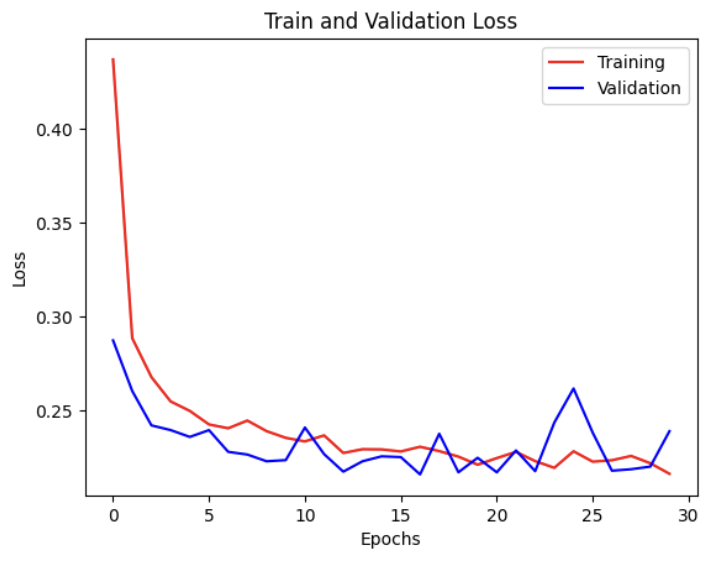
\includegraphics[width=\linewidth]{images/mlpTrainAndValidationLoss.png}
    \caption{Loss during training and validation for the MLP model.}
    \label{fig:mlp_loss_training_validation}
\end{figure}

The training curves of the MLP indicate stable and favorable learning behavior. In the accuracy plot, both the training and validation sets reach values above 90\%, with minor fluctuations in the validation accuracy, possibly due to data variability. The loss plot further supports this observation, showing a consistent decrease in loss for both sets, with no clear signs of overfitting. Overall, the curves suggest that the model generalizes well and maintains a good balance between learning and predictive performance.

\begin{table}[H]
    \centering
    \caption{Classification report for the evaluated model} 
    \label{tab:mlp_classification_report}
    \begin{tabular}{lcccc}
        \toprule
        Class & Precision & Recall & F1-Score & Support \\
        \midrule
        0 (Non-toxic) & 0.81 & 0.86 & 0.84 & 4669 \\
        1 (Toxic)     & 0.86 & 0.81 & 0.83 & 4869 \\
        \midrule
        Accuracy      &      &      & 0.83 & 9538 \\
        Macro Avg     & 0.84 & 0.84 & 0.83 & 9538 \\
        Weighted Avg  & 0.84 & 0.83 & 0.83 & 9538 \\
        \bottomrule
    \end{tabular}
\end{table}

As shown in Table~\ref{tab:mlp_classification_report}, the classification report reveals similar issues to other models such as SVM, XGBoost, and BI-LSTM, where more examples are predicted as “non-toxic.” This model also shows slightly worse performance compared to the previously mentioned models.

\begin{figure}[H]
    \centering
    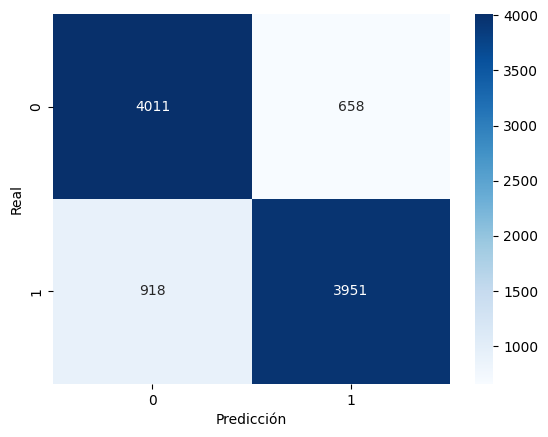
\includegraphics[width=0.45\textwidth]{images/mlp_confusion_matrix.png}
    \caption{Confusion matrix of the MLP model on the test set.}
    \label{fig:mlp_confusion_matrix}
\end{figure}

In Figure~\ref{fig:mlp_confusion_matrix}, the confusion matrix of the MLP model is shown. This matrix confirms that the model has greater difficulty in accurately classifying toxic and non-toxic examples.